\chapter{Metodologia}

descrição das técnicas em detalhes

\section{Amostragem}

\textit{falar sobre a amostragem das Lyraes e Nyquist}

\section{Analise de Fourier}

\subsection{Lomb-Scargle}

\section{Espaço de fase}

Quando uma estrela possui um comportamento periódico, a variação em sua magnitude é representada em ciclos iguais. Cada ciclo é uma fase. Se os ciclos são iguais, não importa qual ciclo nos estamos observando, apenas onde nos estamos no ciclo. Assim, o espaço de fase é uma representação de todos os ciclos observados em apenas uma fase, ou em apenas um ciclo. Assim, os pontos de sobrepõem e formam uma oscilação geral da estrela. Este espaço de fase é calculado pela seguinte expressão,
\begin{equation}
\phi_i = \frac{t_i}{P} - \Big[\frac{t_i}{P}\Big]
\end{equation}
em que $t_i$ é o i-ésimo dado do tempo, $P$ é o período de oscilação da magnitude e a quantidade entre colchetes representa apenas o numero inteiro da divisão. 
%Most of the entropy based methods are based on information entropy. In information theory, entropy is a measure of the uncertainty in a random variable. So, the entropy measures the lack of information of one variable.

%Information theory based methods extract information from the probability density function and so include higher-order statistical moments present in the data whereas Fourier or analysis of variance techniques are based only on second-order statistical analyses. This implies that information theory brings better modeling of the underlying process and robustness to noise and outliers \citep{graB13}.


%Para calcular a entropia condicional, primeiramente é necessário transformar os dados para o espa\c{c}o de fase e normalizar a luminosidade da estrela. Quando os dados são lidos pelo programa, ele gera dois vetores, um com os dados sobre o tempo e outro com os dados sobre a luminosidade da estrela. Para transformar o tempo em fase é necessário dividir cada um dos elementos do vetor tempo pelo período e subtrair o inteiro desta divisão,
%\begin{equation}
%\phi_i = \frac{t_i}{P} - \Big[\frac{t_i}{P}\Big]
%\end{equation}
%assim, temos um novo vetor com os dados da fase. O gráfico que pode ser obtido com os dados da fase e da luminosidade representa a dispersão da série temporal no espa\c{c}o de fase. A entropia condicional é calculada a partir desta dispersão.

%Um exemplo de espa\c{c}o de fase é dado a seguir: 

\begin{figure}[h!]
\centering
\begin{subfigure}{.5\textwidth}
  \centering
  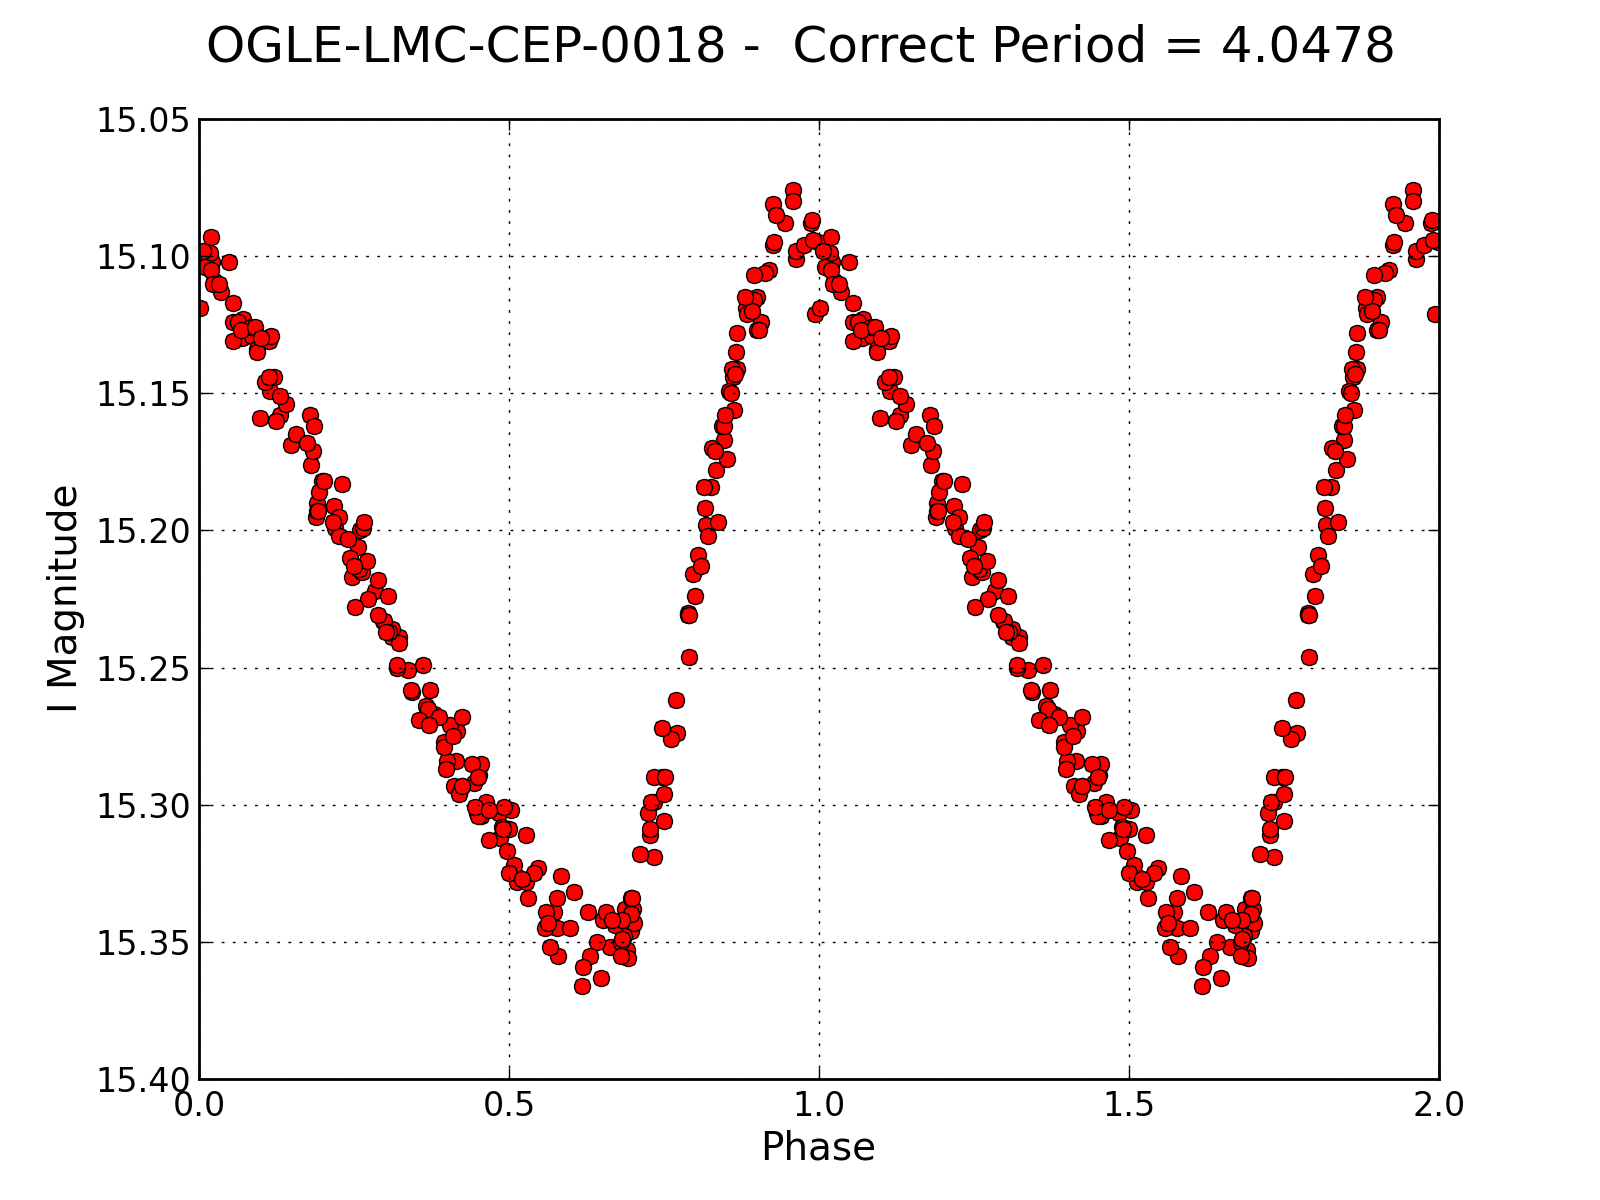
\includegraphics[width=\linewidth]{lightcurve_0018_correct_period.png}
  \caption{Período correto}
  \label{fig:right}
\end{subfigure}%
\begin{subfigure}{.5\textwidth}
  \centering
  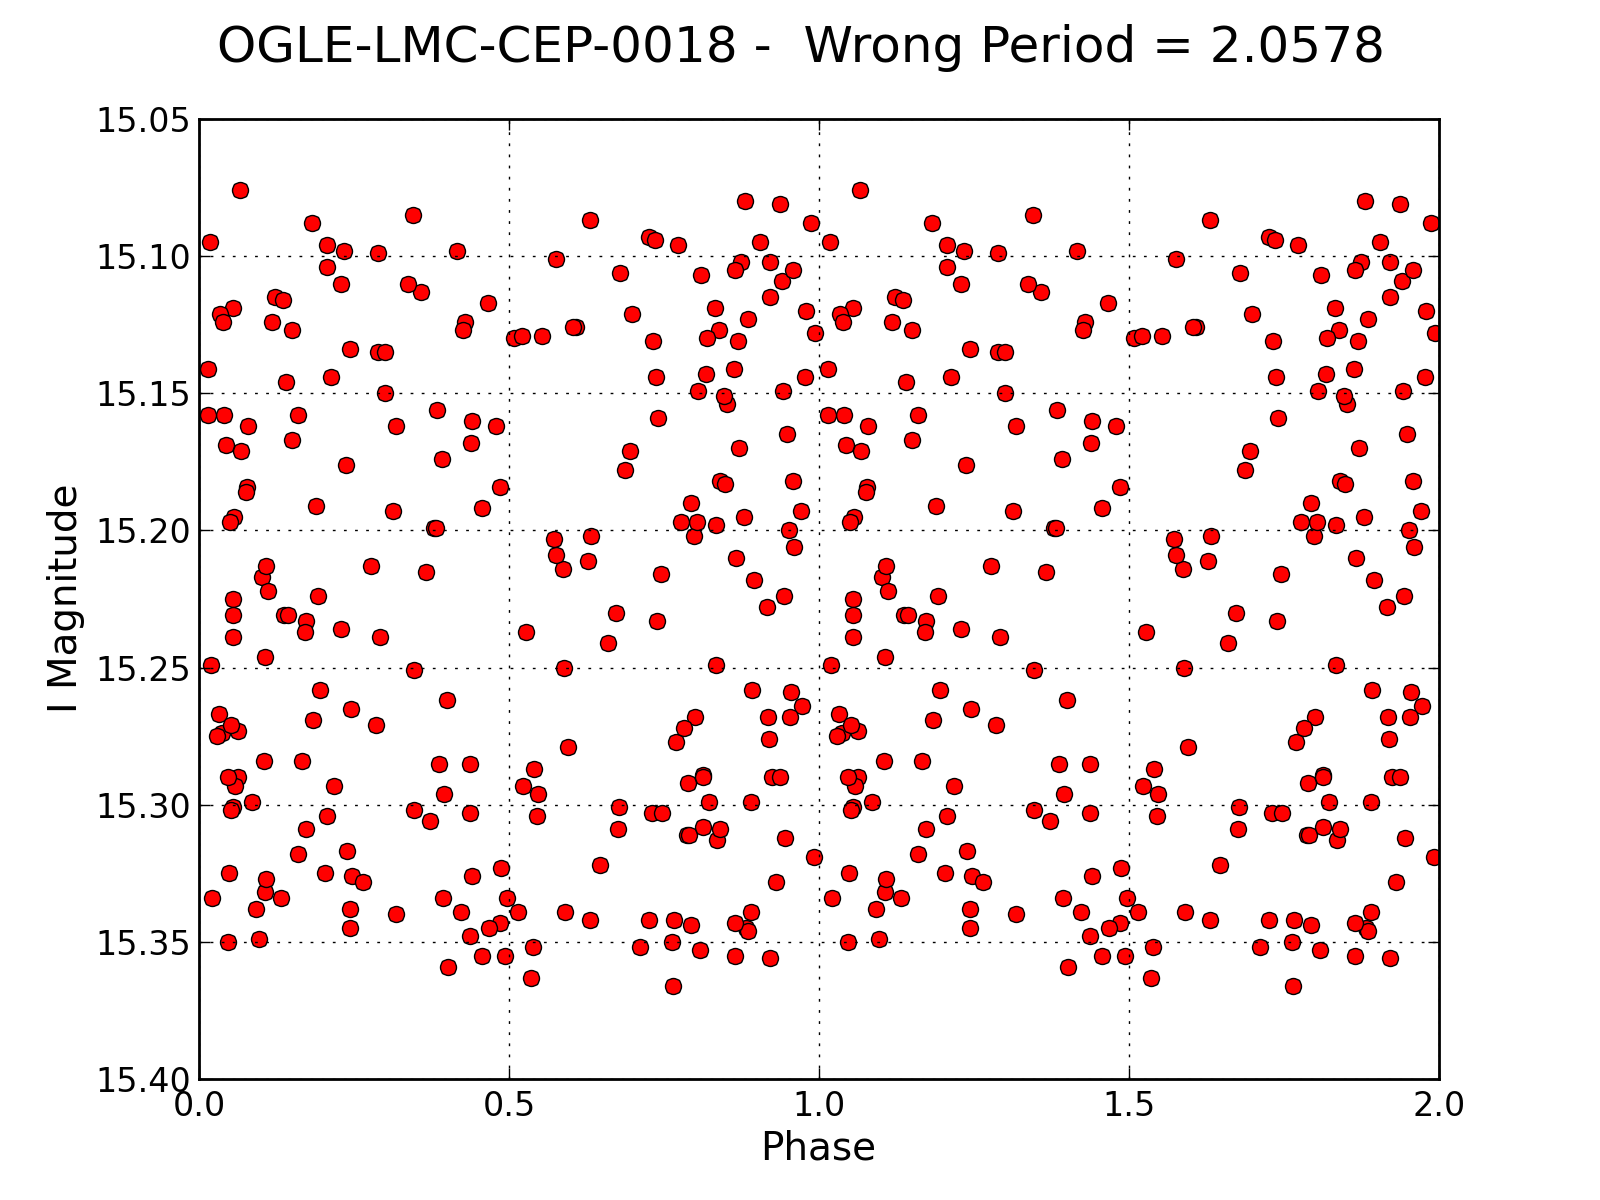
\includegraphics[width=\linewidth]{lightcurve_0018_wrong_period.png}
  \caption{Período errado}
  \label{fig:wrong}
\end{subfigure}
\caption{Exemplos de espa\c{c}o de fase}
\label{fig:exemplo}
\end{figure}

Quando uma série temporal é dividida pelo período correto, será gerado uma dispersão com característica oscilante, como é o caso da figura \ref{fig:right}. Se o período utilizado na transforma\c{c}ão não for o correto, será gerado uma dispersão aleatória, sem forma definida, como mostra a figura \ref{fig:wrong}. 

\subsection{Entropia de Shannon}

Na teoria de informação, a entropia, ou entropia de Shannon, é a medida de incerteza de uma variável. A entropia de Shannon mede a falta de informação do nosso sistema, ou seja, quanto maior o seu valor mais incorreto a variável que estamos medindo. Desta forma, vamos procurar pela minimização da entropia no nosso espaço de fase.

\begin{comment}
Quando uma estrela possui um comportamento periódico, a variação em sua magnitude é representada em ciclos iguais. Cada ciclo é uma fase. Se os ciclos são iguais, não importa qual ciclo nos estamos observando, apenas onde nos estamos no ciclo. Assim, o espaço de fase é uma representação de todos os ciclos observados em apenas uma fase, ou em apenas um ciclo. Assim, os pontos de sobrepõem e formam uma oscilação geral da estrela. Este espaço de fase é calculado pela seguinte expressão,
\begin{equation}
\phi_i = \frac{t_i}{P} - \Big[\frac{t_i}{P}\Big]
\end{equation}
em que $t_i$ é o i-ésimo dado do tempo, $P$ é o período de oscilação da magnitude e a quantidade entre colchetes representa apenas o numero inteiro da divisão. 
%Most of the entropy based methods are based on information entropy. In information theory, entropy is a measure of the uncertainty in a random variable. So, the entropy measures the lack of information of one variable.

%Information theory based methods extract information from the probability density function and so include higher-order statistical moments present in the data whereas Fourier or analysis of variance techniques are based only on second-order statistical analyses. This implies that information theory brings better modeling of the underlying process and robustness to noise and outliers \citep{graB13}.


%Para calcular a entropia condicional, primeiramente é necessário transformar os dados para o espa\c{c}o de fase e normalizar a luminosidade da estrela. Quando os dados são lidos pelo programa, ele gera dois vetores, um com os dados sobre o tempo e outro com os dados sobre a luminosidade da estrela. Para transformar o tempo em fase é necessário dividir cada um dos elementos do vetor tempo pelo período e subtrair o inteiro desta divisão,
%\begin{equation}
%\phi_i = \frac{t_i}{P} - \Big[\frac{t_i}{P}\Big]
%\end{equation}
%assim, temos um novo vetor com os dados da fase. O gráfico que pode ser obtido com os dados da fase e da luminosidade representa a dispersão da série temporal no espa\c{c}o de fase. A entropia condicional é calculada a partir desta dispersão.

%Um exemplo de espa\c{c}o de fase é dado a seguir: 

\begin{figure}[h!]
\centering
\begin{subfigure}{.5\textwidth}
  \centering
  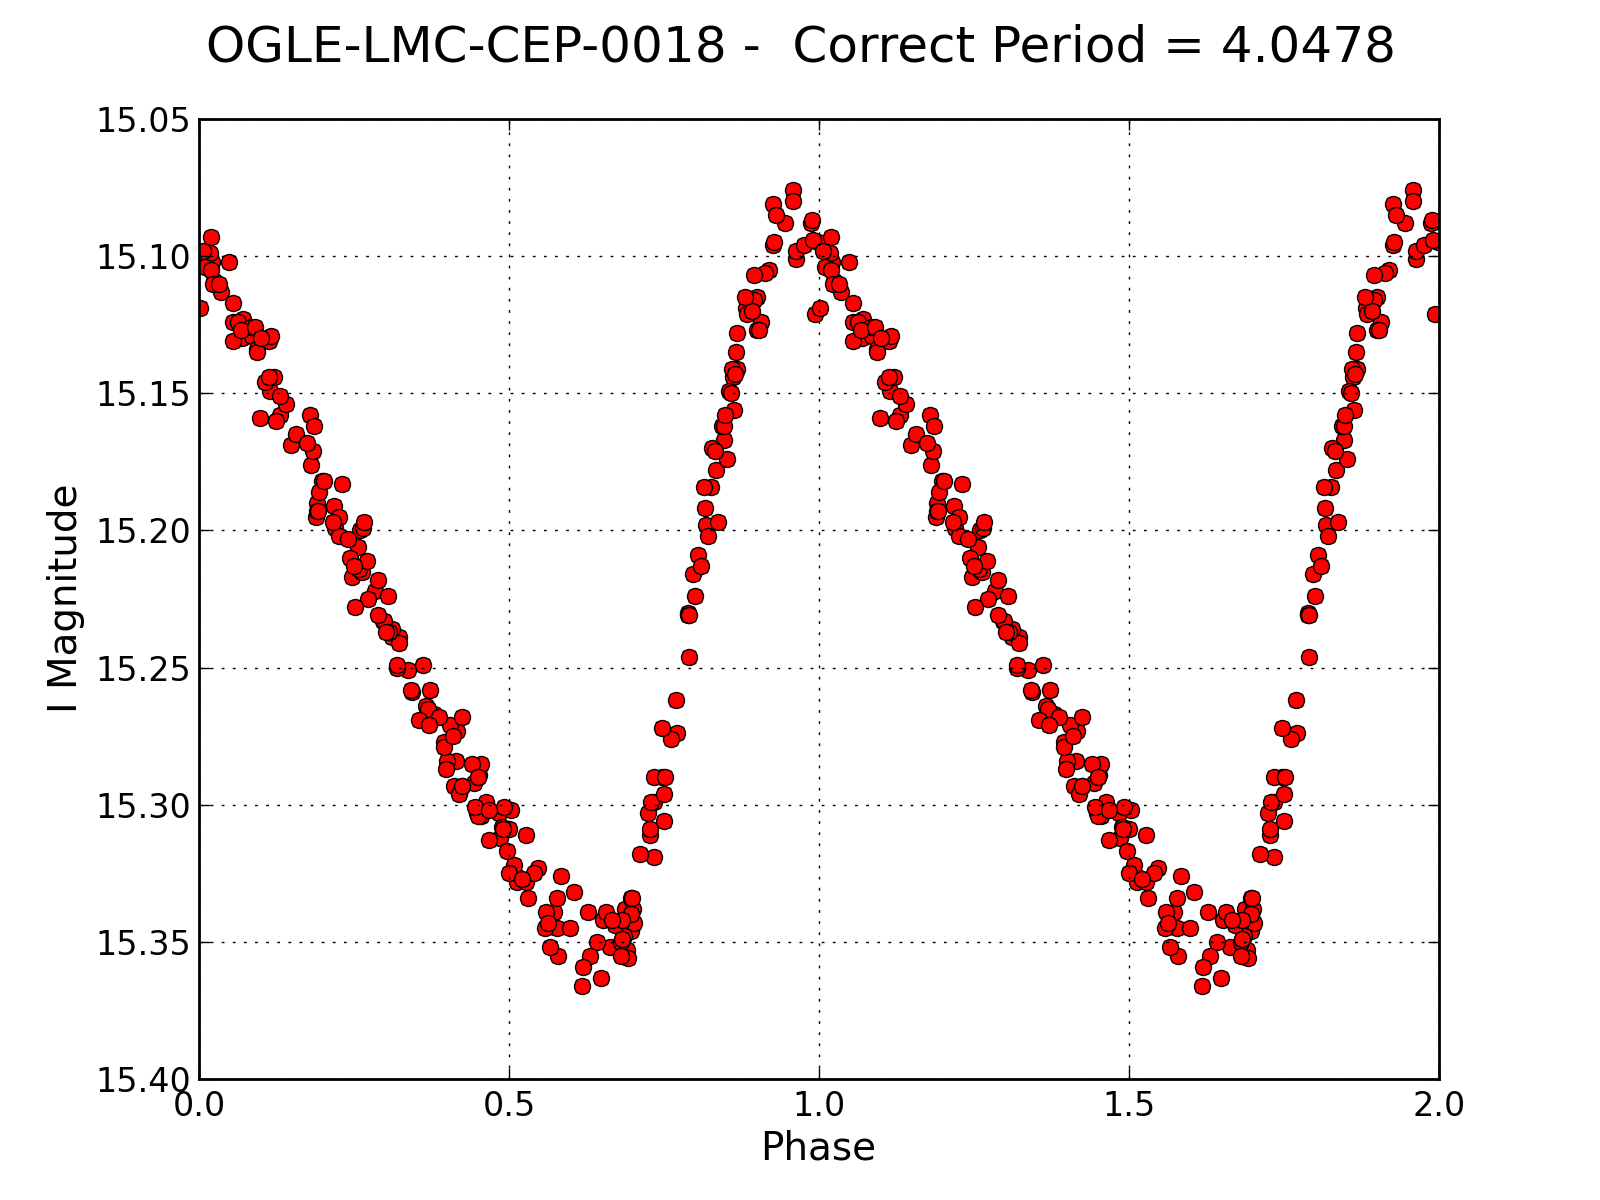
\includegraphics[width=\linewidth]{lightcurve_0018_correct_period.png}
  \caption{Período correto}
  \label{fig:right}
\end{subfigure}%
\begin{subfigure}{.5\textwidth}
  \centering
  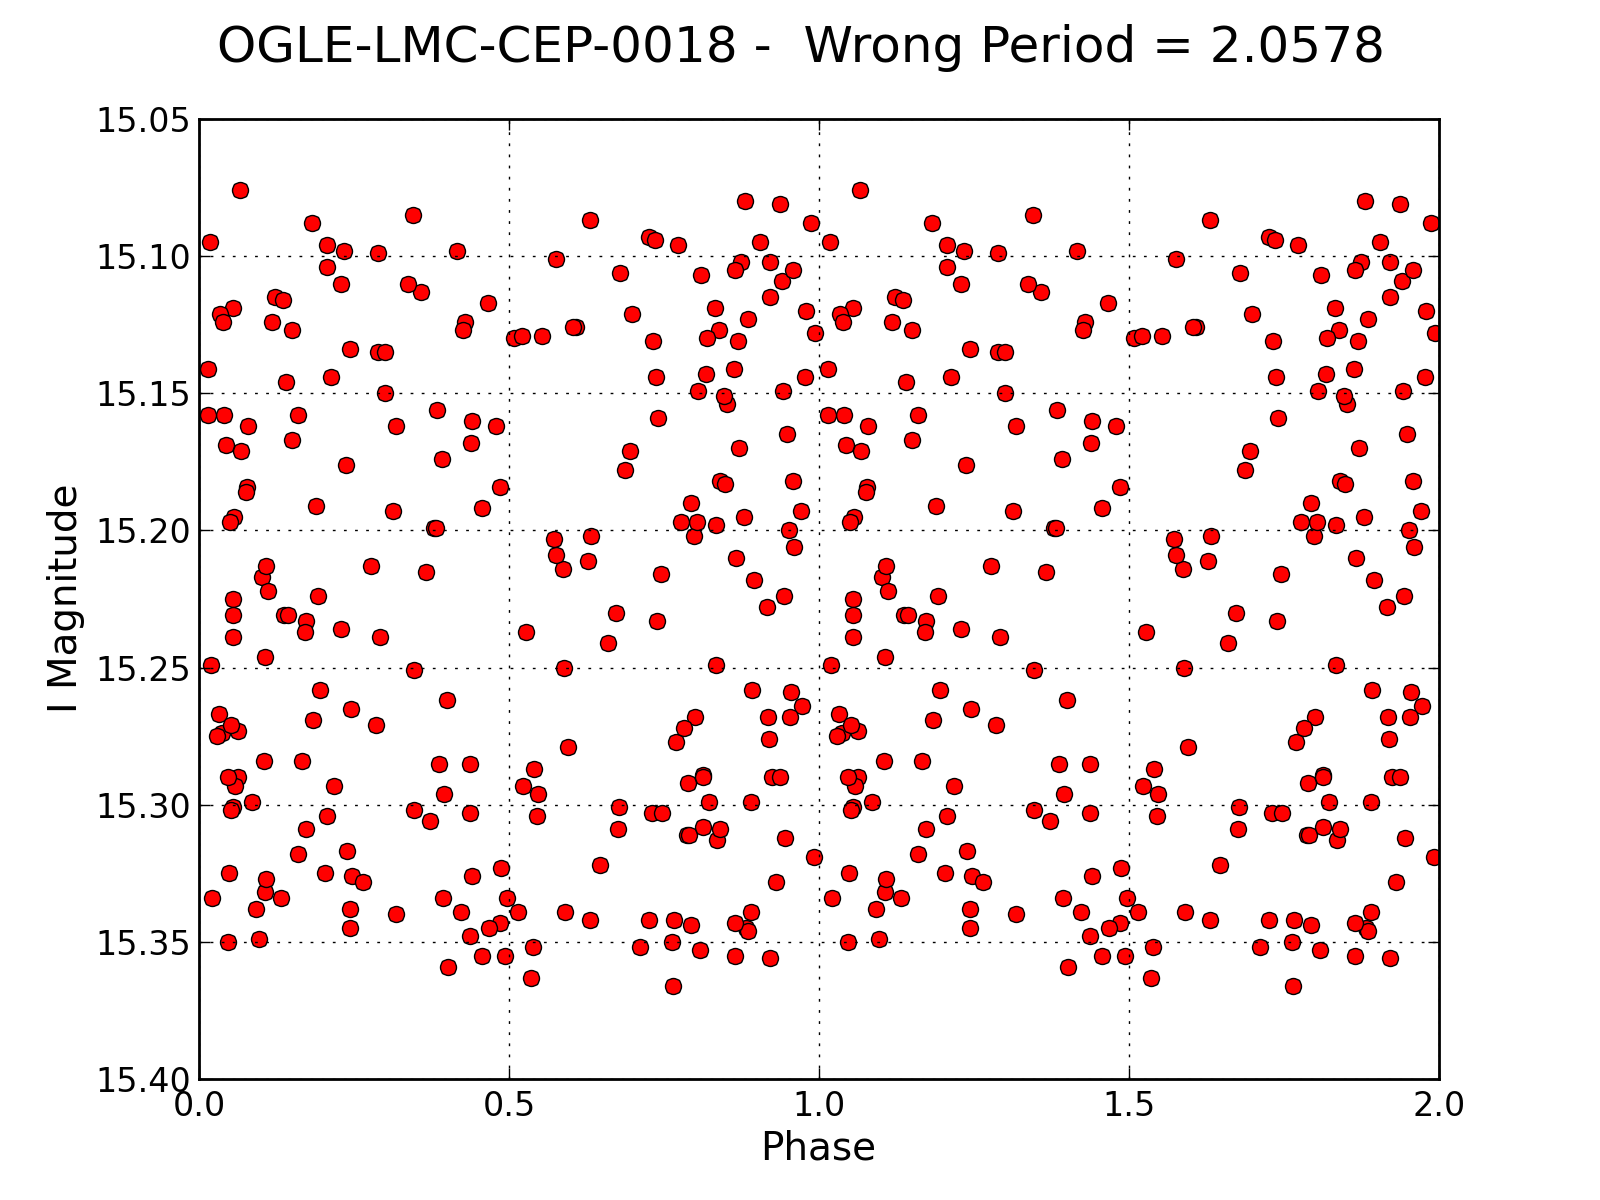
\includegraphics[width=\linewidth]{lightcurve_0018_wrong_period.png}
  \caption{Período errado}
  \label{fig:wrong}
\end{subfigure}
\caption{Exemplos de espa\c{c}o de fase}
\label{fig:exemplo}
\end{figure}

Quando uma série temporal é dividida pelo período correto, será gerado uma dispersão com característica oscilante, como é o caso da figura \ref{fig:right}. Se o período utilizado na transforma\c{c}ão não for o correto, será gerado uma dispersão aleatória, sem forma definida, como mostra a figura \ref{fig:wrong}. 

\end{comment}

Podemos observar que, no caso da figura \ref{fig:right}, os pontos se sobrepõem e formam uma curva. Assim, fazendo reparti\c{c}ões no dimensão da fase e da magnitude, podemos calcular a probabilidade dos pontos estarem localizados em cada um dos quadrados formados por estas reparti\c{c}ões em rela\c{c}ão a coluna em que eles estão e somá-los para obter uma grandeza. Esta grandeza é a entropia condicional, que é calculada pela seguinte formula \citep{ce},

\begin{equation}
H_c = \sum_{i,j} p(m_i,\phi_j)\ln \Big(\frac{p(\phi_j)}{p(m_i,\phi_j)}\Big)
\end{equation}
onde $p(m_i,\phi_j)$ é a probabilidade de ocupa\c{c}ão na $i$-ésima reparti\c{c}ão da magnitude e na $j$-ésima reparti\c{c}ão da fase e $p(\phi_j)$ é a probabilidade de ocupa\c{c}ão na $j$-ésima reparti\c{c}ão da fase. No caso de reparti\c{c}ões retangulares, %a probabilidade de ocupa\c{c}ão
\begin{equation}
p(\phi_j) = \sum_i p(m_i,\phi_j)
\end{equation}

A entropia de Shannon mede a falta de informa\c{c}ão do sistema, ou seja, quanto maior o seu valor, mais incorreto o período. Por isso que buscamos a minimiza\c{c}ão da entropia.
Considerando estes dois exemplos, a probabilidade de de ocupa\c{c}ão das reparti\c{c}ões é menor na figura \ref{fig:right} do que na figura \ref{fig:wrong}. O menor valor de entropia condicional é associado ao período mais provável da estrela \citep{ce}. 

\section{Algoritmo}

Foi desenvolvido um algoritmo em Python3 para calcular a entropia condicional de dados pertencentes ao \href{http://ogledb.astrouw.edu.pl/~ogle/CVS/}{Catálogo OGLE-III de estrelas variáveis}. Os dados são obtidos no formato .dat e possuem três colunas que significam tempo, magnitude e erro. Um exemplo de arquivo pode ser visto na tabela \ref{tab:dados}.
\begin{center}
\captionof{table}{Exemplo de dados}
\begin{tabular}{c|c|c} 
\hline 
Tempo & Magnitude & Erro \\ 
\hline 
2165,85271 & 15,130 & 0,007 \\ 
%\hline 
2183,83450 & 15,326 & 0,008 \\ 
2238,62899 & 15,102 & 0,007 \\ 
$\vdots$ & $\vdots$ & $\vdots$ \\
\hline 
\end{tabular} 
\label{tab:dados}
\end{center}

Um loop é iniciado e para o primeiro valor do vetor período, o tempo é transformado em fase. São feitas as reparti\c{c}ões para este espa\c{c}o de fase e são contabilizados a quantidade de pontos em cada reparti\c{c}ão. Então a entropia condicional é calculada e este valor é armazenado num vetor entropia. O mesmo é feito para o próximo período do vetor período até que sejam calculados a entropia para todos os dados deste vetor. No fim, o algoritmo indica o menor valor do vetor entropia e qual período esta relacionado com este valor. A figura \ref{fig:flow} apresenta um fluxograma do algoritmo.

\begin{figure}[!hb]
\centering
	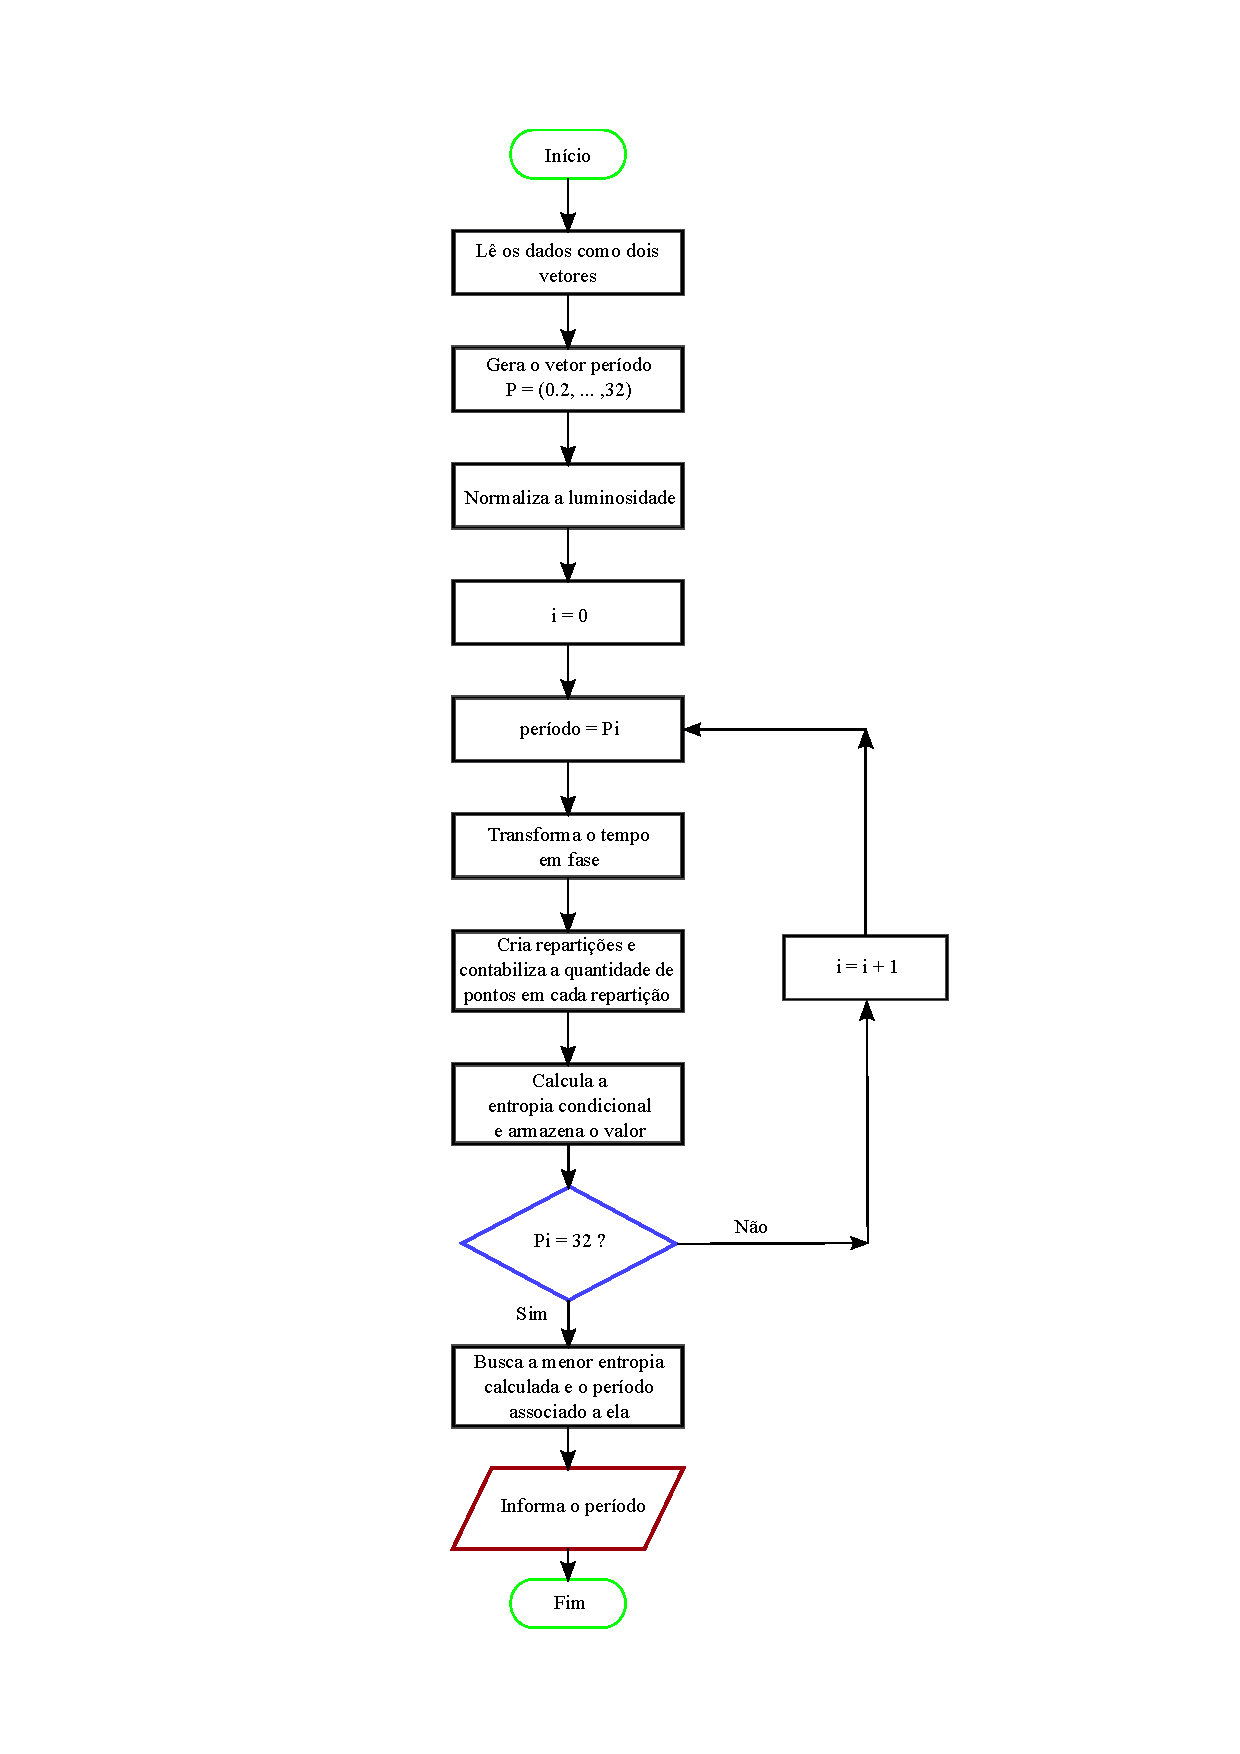
\includegraphics[scale=.6]{drawing.pdf}
	\caption{Fluxograma do algoritmo}
	\label{fig:flow}
\end{figure}
